% presentation with pdflatex + foils package
% http://robotics.stanford.edu/~gerkey/tools/saynotopowerpoint.html

% use the foils document class, with large fonts and landscape orientation
\documentclass[20pt,landscape,a4paper]{foils}

% setup the page geometry for landscape and use maximum screen real estate
\usepackage[pdftex]{geometry}
\geometry{headsep=2.0em,hscale=0.80}

% Define page margins
\setlength{\topmargin}{-1.0in}
%\addtolength{\oddsidemargin}{-0.5in}
%\addtolength{\textwidth}{1.0in}
\setlength{\oddsidemargin}{-0.5in}
\setlength{\textwidth}{10.0in}
\setlength{\textheight}{7in}
\setlength{\foilheadskip}{-0.5in}

% boldmath, serve per fare le lettere greche in bold
\usepackage{bm}

% title, author, date
\title{Bayes-swarm\\bayesian web spidering}
\author{Associazione BayesFor\\info@bayesfor.eu}
\date{27 ottobre 2007}

% the contents of \MyLogo are placed at the bottom center on the title slide
% and in the bottom left of other slides
\MyLogo{Associazione BayesFor, Bayes-swarm}

% basic things that we need are below
\usepackage[italian]{babel}
\usepackage[utf8]{inputenc}
\usepackage{hyperref}
\hypersetup{
  pdftitle={Bayes-swarm, bayesian web spidering and information retrieval},
  pdfauthor={Matteo Zandi, Riccardo Govoni},
  pdfsubject={Bayes-swarm, research project which aims to spider web sources and extract data with bayesian models},
%  pdfpagemode={FullScreen},
  pdfborder={0 0 0}
}
\usepackage{graphicx}

% set slide command
\newcommand{\slide}[1]{\foilhead{#1}}

% document
\begin{document}

\LogoOff
\maketitle
\begin{center}
  
\includegraphics{./figures/linuxday2007.png}
\end{center}

\slide{Cos'è Bayesfor?}
\LogoOn
\noindent
Una associazione che si propone di promuovere e realizzare ricerche,
studi o sperimentazioni in materia di analisi dei dati e utilizzo di
tecniche statistiche

\begin{center}
  http://bayesfor.eu
\end{center}

Membri:
\begin{itemize}
  \item Bonazzi Alessandro (alessandro.bonazzi@bayesfor.eu)
  \item Brunori Paolo (paolo.brunori@bayesfor.eu)
  \item Govoni Riccardo (riccardo.govoni@bayesfor.eu)
  \item Lampronti Giulio (giulio.lampronti@bayesfor.eu)
  \item Zandi Matteo (matteo.zandi@bayesfor.eu).
\end{itemize}

\begin{center}
http://code.google.com/p/bayes-swarm/wiki/AboutUs
\end{center}

\slide{... e Bayes-swarm?}
\noindent
E' un progetto della associazione Bayesfor, che ha l'obiettivo di fare spidering
di fonti sul web con lo scopo di estrarre informazioni come ad esempio:
\begin{itemize}
  \item Correlazione tra parole nel tempo
  \item Associazioni tra parole nelle fonti
  \item Correlazione tra uso di parole e notizie
  \item Correlazione tra uso di parole e mercati finanziari
\end{itemize}

\begin{center}
  http://bayes-swarm.googlecode.com
\end{center}

\slide{Come funziona}
\begin{itemize}
\item Lista di fonti (siti di quotidiani italiani ed esteri, agenzie
di stampa, feed rss, etc)
\item Lista di parole "interessanti" (per ora, ma non per molto)
\item Ruby + gemme (ferret, hpricot, scrubyt, etc)
\item Mysql, database in cui sono salvate tutte le informazioni
\end{itemize}

\slide{Alcuni numeri}
\begin{itemize}
\item 7 fonti (times, guardian, euronews, ny times, al jazeera, etc)
\item 22 pagine, circa 3 per fonte (pagina principale, economica, finanziaria, etc)
\item 87 parole interessanti (china, india, bush, iraq, terror, muslim, etc)
\item circa 1000 occorrenze a settimana
\item ... attualmente a dimensioni prototipali, puo' scalare a volumi molto maggiori
\end{itemize}

\slide{Le fasi del processo di estrazione}
\begin{center}
  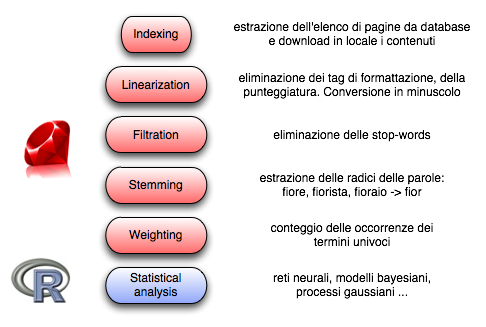
\includegraphics{./figures/elab_phases.png}
\end{center}
Il processo di estrazione utilizza un sistema modulare facilmente estendibile,
basato sul concetto di ETL (Extact, Transform and Load) tipico dei datawarehouse.
%\begin{center}
%    http://www.miislita.com/information-retrieval-tutorial/indexing.html
%\end{center}

%\slide{Le fasi del processo di estrazione (continua)}
%\begin{center}
%    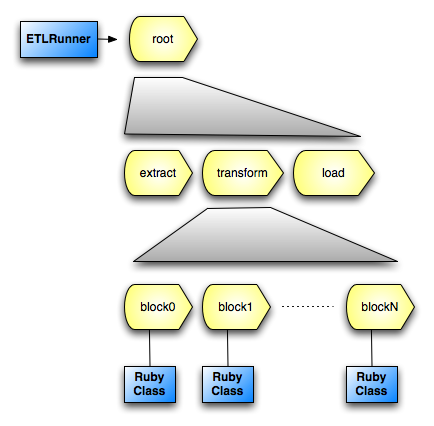
\includegraphics{./figures/etl_chains.png}
%\end{center}

\slide{Grafico serie storica Bindi e Letta}
\begin{center}
  \includegraphics{./figures/timeseries_bindi-letta.pdf}
\end{center}
\noindent
\begin{itemize}
\item XXX
\end{itemize}

\slide{Grafici di Veltroni e PD}
\begin{center}
  \includegraphics{./figures/timeseries-scatter_veltroni-pd.pdf}
\end{center}
\noindent
\begin{itemize}
  \item Veltroni e PD tendono a mostrarsi congiuntamente?
  \item Coefficiente di correlazione $\cong 0.79$
\end{itemize}

\slide{Applicazione di modelli statistici 1/3}
%\begin{center}
%  \includegraphics{./figures/lm_hw_gp.pdf}
%\end{center}
\noindent
\begin{itemize}
  \item Least squares: regressione semplice, presuppone una dipendenza lineare del tipo $y=a+bx$.
  \item Exponential smoothing: media di $n$ osservazioni precedenti con peso decrescente in funzione della distanza da oggi.
  \item Processo gaussiano: i parametri del modello non sono fissi, dipendono dal tempo.
\end{itemize}

\slide{Applicazione di modelli statistici 2/3}
%\begin{center}
%  \includegraphics{./figures/bi_lm_gp.pdf}
%\end{center}
\noindent
\begin{itemize}
  \item Least squares: stiamo ipotizzando che tra china e india esista
  una dipendenza fissa.
  \item Processo gaussiano: il modello di dipendenza varia in funzione
  del numero di volte in cui le parole sono citate.
\end{itemize}

\slide{Applicazione di modelli statistici 3/3}
\begin{center}
  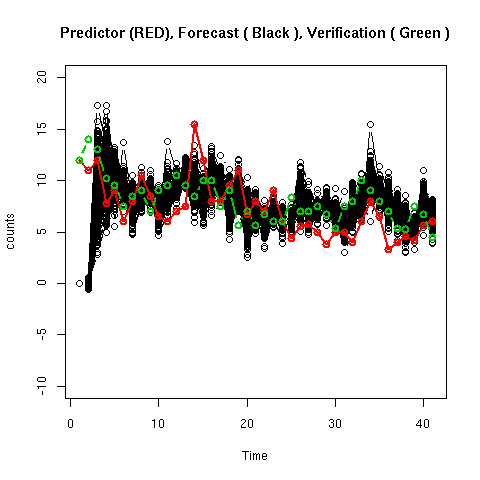
\includegraphics[width=0.4\hsize]{./figures/neural-prediction.png}
  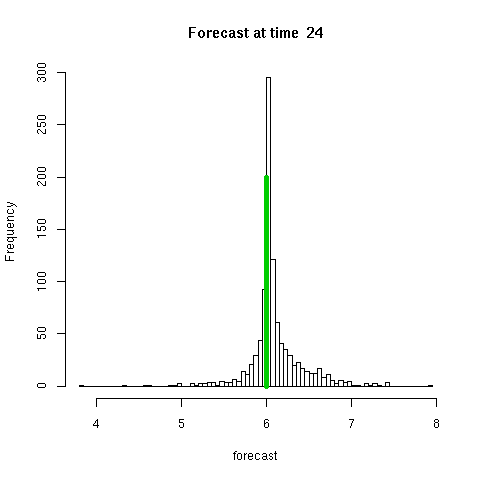
\includegraphics[width=0.4\hsize]{./figures/neural-hist.png}
\end{center}
\noindent
Neural network:
\begin{itemize}
  \item{Il modello è indotto dalla misurazione dei dati.}
  \item{Il processo di modellizzazione implica il riconoscimento di
  regolarità (pattern) in modo da ottenere una efficace rappresentazione
  dei dati utilizzabile per fare previsioni.}
\end{itemize}

\slide{Teoria dei grafi}
\noindent
Utilizzo dei legami parola - pagina per creare grafi di relazioni, da cui estrarre relazioni dirette tra parole che appaiono nello stesso contesto (quando si parla di questo, si parla anche di...)
\begin{center}
  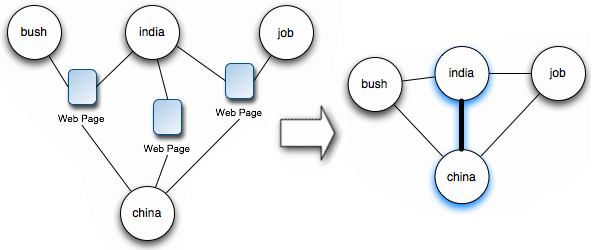
\includegraphics{./figures/graph_compression2.png}
\end{center}
E' alla base dei sistemi di advertising piu' famosi: Amazon.com, ('chi ha comprato questo, ha comprato anche...'), Google Adwords ('se hai fatto questa ricerca, forse sei interessato anche a ...')

\slide{Teoria dei grafi (continua)}
\begin{center}
  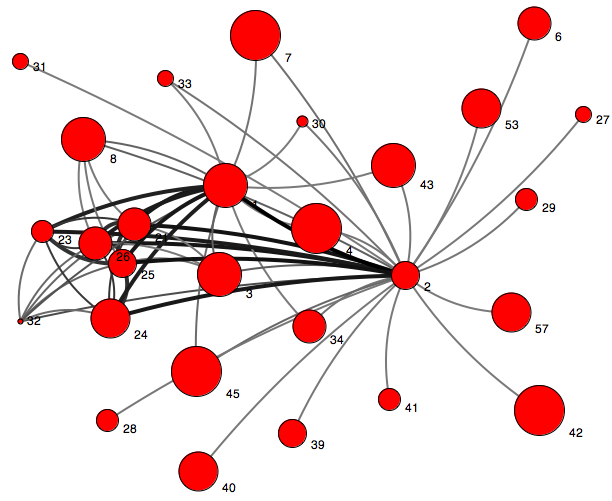
\includegraphics[width=0.4\hsize]{./figures/graphs.png}
\end{center}
\noindent
Ogni parola costituisce una 'stella', a parole con frequenza maggiore
sono associate stelle di dimensione maggiore. Ogni parola è connessa alle
altre se sono state almeno una volta nella stessa pagina, la connessione
è tanto più marcata quante più volte le parole si sono trovate nella stessa pagina.

\slide{Teoria dei grafi e Clustering}
\noindent
Applicare tecniche di clustering e raggruppamento (k-means, hierarchical, edge-betweenness) aiuta a identificare quali parole sono contestuali tra loro e quali invece irrilevanti.

\begin{center}
  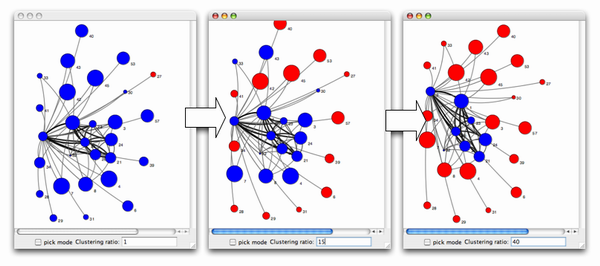
\includegraphics{./figures/graph_clustering.png}
\end{center}

\slide{Da qui in avanti}
\begin{itemize}
  \item aumento del corpus di dati oggetto di analisi
  \item analisi sulle forme di distribuzione dell'informazione derivanti dal web 2.0: i feed rss
  \item sperimentazione di altre tecniche statistiche (SVD, ...)
  \item sperimentazione su corpus di dati preesistenti di grandi dimensioni (il dataset Enron)
\end{itemize}

\slide{Grazie per l'attenzione}
\noindent
\begin{center}
  http://bayesfor.eu\\http://bayes-swarm.googlecode.com

  \huge{domande?}
\end{center}

\slide{Backup}

\slide{Distribuzione gaussiana e processo gaussiano a confronto}
\textbf{Distribuzione Gaussiana}
\[X \sim N(\mu, \sigma)\]
Distribuzione statistica per eccellenza, ha densità pari a
\[ P(X=x)= \frac{1}{\sigma\sqrt{2\pi}} \,\exp\biggl( -\frac{(x- \mu)^2}{2\sigma^2}\biggr)\]

\textbf{Processo gaussiano}
\[ X(t) \sim N(\mu(t), \sigma(t)) \]
Processo stocastico $X(t)_{t \in T}$ tale per cui ogni combinazione
di $X(t)$ considerata è distribuita normalmente.
\[ \left[ \begin{array}{c} x_{n+1} \\ \bm{x}_{1:n} \end{array} \right]
  \sim N\left( \left[ \begin{array}{c} m(t_{n+1}) \\ m(\bm{t}_{1:n}) \end{array} \right] ,
    \left[ \begin{array}{cc} k & \bm{k}^T \\ \bm{k} & \bm{K} \end{array} \right]
  \right)
\]
Una delle possibili matrici di covarianza è definita come $k(x_i,x_j)=e^{-\frac{1}{2 \sigma}(x_i-x_j)^2}$
\end{document}
